\documentclass [12pt]{article}
\usepackage{graphicx}
\usepackage{amstext,verbatim,alltt}
\usepackage{moreverb}
\setlength{\textwidth}{6.5in}
\setlength{\oddsidemargin}{0in}
\setlength{\evensidemargin}{0in}
\begin{document}

\title{The BLASBench Report}
\author {Philip J. Mucci \\
	Kevin S. London \\
	John Thurman \\
        {\tt mucci@cs.utk.edu} \\
	{\tt london@cs.utk.edu} \\
	{\tt thurman@cs.utk.edu}}
\date{February, 1999}

\maketitle

\section{Introduction}

BLASBench is a benchmark designed to evaluate the performance of some
kernel operations of different implementations of the BLAS
routines. The BLAS are the Basic Linear Algebra Subroutines and are
found in some form or another on most vendors' machines. The BLAS were
initially developed as part of LAPACK. Their goal was to provide a
standardized API for common Vector-Vector, Vector-Matrix and
Matrix-Matrix operations. A version of the BLAS is
available from Netlib at {\tt http://www.netlib.org}. This version is
subsequently referred to as the reference version. The reference BLAS
are completely unoptimized Fortran codes intended as a reference for
correctness to the vendors.

As of November, 1998 BLASBench has been integrated into the LLCbench benchmarking suite.

\section{Goals of BLASBench}

BLASBench aims to provide the following:

\begin{itemize}
\item Evaluate the performance of the BLAS routines in MFLOPS/sec.
\item Provide
information for performance modeling of applications that make heavy
use of the BLAS.
\item  Evaluate compiler efficiency by comparing
performance of the reference BLAS versus the hand-tuned BLAS provided
by the vendor.
\item Validate vendor claims about the numerical performance 
of their processor.
\item Compare against peak cache performance to establish bottleneck, memory
or CPU.
\end{itemize}

\section{Description}

BLASBench currently benchmarks the three most common routines in the
BLAS. They are:

\begin{itemize}
\item {\em AXPY} - Vector addition with scale
\item {\em GEMV} - Matrix-vector multiplication with scale
\item {\em GEMM} - Matrix-Matrix multiplication with scale
\end{itemize}

The benchmark can run in either single or double precision. This is
important as many systems cannot sustain the additional memory
bandwidth required by using double precision data. The
test space is highly tunable, as are some of the metrics BLASBench reports. 
It reports its results in MFLOPS/sec and MB/sec. These
numbers are not computed from hardware statistics, but rather from the
absolute operation and memory reference count required by each
algorithm.

\section{How it works}

BLASBench is a C program that calls BLAS routines written in
Fortran, the reason for this being that we wish to perform dynamic
memory allocation.
%control how the
%memory is allocated and aligned. Improper alignment of the vectors and
%arrays can result in exceedingly poor performance due to cache line
%conflicts and page misses. Here we align the arrays properly, in a
%portable fashion, as our target audience will often have this
%performed either implicitly through compiler options or explicitly by
%padding their COMMON blocks. 
For each test, BLASBench allocates its
memory in such a way that the total amount of memory taken up by each
test is less than or equal to the nearest power of two. The rationale
for this is that our cache sizes are always in a power of two. Once
the memory is allocated, the arrays are initialized, and the test is
run for a certain number of iterations. By default, the iteration
count is not constant over each problem size. BLASBench trys to keep
the amount of data touched by each run constant. This means that
larger problem sizes run for fewer iterations. The effect of this
is that the run time for each size is approximately
constant. BLASBench provides an option to keep the iteration count
constant across all tests. After each size is tested, the cache is
flushed and BLASBench either proceeds to the next size or repeats that
size, depending on the options given to the program. BLASBench allows
you to repeat each size any number of times. This could be used to
validate the numbers from each size on a time-shared
system. By default, BLASBench calls the BLAS routines with the leading
dimension of each array or vector set to the exact size of that
vector. This means that the BLAS routines operate on the entire data
set. Frequently however, BLAS routines are called upon smaller
portions of larger arrays and matrices, thus an option is provided to
keep the leading dimension constant among every test. In this case,
BLASBench allocates the largest possible data set, and simply changes
the working set size passed to each BLAS routine.

\section{Using BLASBench}

\subsection{Obtain the Distribution}

BLASBench is now found in the LLCbench distribution.
The latest release of LLCbench can always be found through the original author's homepage at \\
{\tt http://icl.cs.utk.edu/projects/llcbench}. \\

Now unpack the installation using {\tt gzip} and {\tt tar}.

\begin{verbatim}
kiwi> gzip -dc llcbench.tar.gz | tar xvf -
kiwi> cd llcbench
kiwi>  ls
Makefile     cachebench/  index.html   mpbench/     sys.def@
blasbench/   conf/        user.def     results

\end{verbatim}

\subsection{Build the Distribution}

First we must configure the build for our machine, OS and BLAS libraries. All
configurations support the reference BLAS if available. Before configuration 
{\tt make} with no arguments lists the possible targets.

\begin{verbatim}
kiwi> make
Please use one of the following targets:

        solaris sunos5
        sun sunos4
        sgi-o2k o2k
        linux-mpich
        linux-lam
        alpha
        t3e
        ppc ibm-ppc
        pow2 ibm-pow2
        reconfig (to bring this menu up again)

After configuration, please check the VBLASLIB variable in 
sys.def and make sure that it is pointing to the vendor BLAS
library if one exists.

\end{verbatim}

Configure the build. Here, we are on a Solaris workstation.

\begin{verbatim}
kiwi> make solaris
ln -s conf/sys.solaris sys.def

\end{verbatim}

BLASBench's default runtime variable values are contained in the file {\tt make.def} and may
be modified there.

Examine the {\tt sys.def} file to ensure proper compiler flags and paths to
the different BLAS libraries.  The BLASLIB variable should contain the
absolute path to the reference BLAS library and the VBLASLIB variable
should contain the absolute path to the vendor's BLAS library. If one
or the other is not available, just leave it blank and that specific
executable will not be generated. \\

Now type make to get options for building a benchmark.

\begin{verbatim}
kiwi> make
Please use one of the following targets:

For all three : bench, run, graphs
For Blasbench : blas-bench, blas-run, blas-graphs
For Cachebench: cache-bench, cache-run, cache-graphs
For MPbench   : mp-bench, mp-run mp-graphs

\end{verbatim}

Now build BLASBench.  Depending on whether or not both BLASLIB and VBLASLIB are set,
one or two executables will be generated.

\begin{verbatim}
kiwi> make blas-bench
cd blasbench; make blasbench; make vblasbench
/opt/SUNWspro/bin//cc -fast -dalign -DREGISTER -xarch=v8plusa -c bb.c
if [ -f "/src/icl/LAPACK_LIBS/blas_SUN4SOL2.a" ]; then /opt/SUNWspro/bin//f77 -xarch=v8plusa
-o blasbench bb.o /src/icl/LAPACK_LIBS/blas_SUN4SOL2.a -xlic_lib=sunperf; fi;
/opt/SUNWspro/bin//f77 -xarch=v8plusa -o vblasbench bb.o  -xlic_lib=sunperf

\end{verbatim}

\subsection{Running BLASBench}

BLASBench can be run by hand, but it is intended to be run through the
makefile. Running it via the makefile automates the collection and
presentation process. By default, the makefile runs both executables
with the arguments {\tt -c -o -e 1 -i 10 -x 2 -m 24}. This says that the iteration count
should be constant, the output should be reported in MFLOPS/sec, each
size should be repeated only once, the iteration count should be
set to ten, two measurements are taken betwen every problem size value that is a power of two, 
and the maximum problem size tested is $2 ^{24}$ bytes. You can change the default settings 
by changing the variables in {\tt make.def} after you have configured the distribution.

\begin{verbatim}
kiwi> make blas-run
cd blasbench; make run
mkdir results
if [ -x blasbench ]; then blasbench  -i 10 -e 1 -m 24 -x 2 -c -d -o -v > results/daxpy.dat; fi
if [ -x blasbench ]; then blasbench  -i 10 -e 1 -m 24 -x 2 -c -d -o -a > results/dgemv.dat; fi
if [ -x blasbench ]; then blasbench  -i 10 -e 1 -m 24 -x 2 -c -d -o -t > results/dgemm.dat; fi
.
.
.
Now do a 'make blas-graphs'.

\end{verbatim}

{/em make blas-graphs} will package up the datafiles for
analysis on another machine.  If Gnuplot is present, it will also generate 
the graphs in place and package them separately.

\begin{verbatim}
kiwi>make graphs
Z=`hostname`; cd results; for i in saxpy daxpy sgemv dgemv sgemm dgemm; do if [ -r $.dat ]; then mv $i.dat $i-$Z.dat; fi; done;
Z=`hostname`; cd results; for i in vsaxpy vdaxpy vsgemv vdgemv vsgemm vdgemm; do if  -r $i.dat ]; then mv $i.dat $i-$Z.dat; fi; done;
Z=`hostname`; cd results; mv info.dat $Z.info
Z=`hostname`; Y=`uname -m`; X=`uname -sn`; sed -e "s|TITLE|UTK BLAS performance for Z: $Y|g" < blasgraph.gp > results/custom.gp; echo "plot \"daxpy-$Z.dat\" title 'saxp' with linespoints \\" >> results/custom.gp; for i in dgemv dgemm; do echo ", \"$i-$.dat\" title '$i' with linespoints \\" >> results/custom.gp; done;
.
.
.
Z=`hostname`; cd results; tar cvf $Z-bp-datafiles.tar *.dat *.gp *.info; 
.
.
.
Z=`hostname`; cd results; tar cvf $Z-bp-graphs.tar *.ps
blasperf.ps
compare.ps
vblasperf.ps

If you don't have GNUplot, you can make the graphs on another machine
using the blasbench/results/kiwi-bp-datafiles.tar file.


\end{verbatim}

Using Gnuplot to create the graphs will result in either 1 or 3 graphs. Each graph contains the
performance in megaflops of all three operations. They are named as
follows:

\begin{itemize}
\item blasperf.ps - Postscript file of the reference BLAS.
\item vblasperf.ps - Postscript file of the vendor's BLAS.
\item compare.ps - Comparison of the two.
\end{itemize}

\subsection{Arguments to BLASBench}

This is the BLASBench arguement list from the command line help.  The defaults listed are
for direct execution of the benchmark (not the defaults for execution through the makefile).

\begin{verbatim}
kiwi> blasbench -h
Usage: blasbench [-vatsco -x # -m # -e # -i #]
         -v AXPY dot product benchmark
         -a GEMV matrix-vector multiply benchmark
         -t GEMM matrix-matrix multiply benchmark
         -s Use single precision floating point data
         -c Use constant number of iterations
         -o Report Mflops/sec instead of MB/sec
         -x Number of measurements between powers of 2.
         -m Specify the log2(available physical memory)
         -e Repeat count per cache size
         -l Hold LDA and loop over sizes of square submatrices
         -d Report dimension statistics instead of bytes
         -i Maximum iteration count at smallest cache size

Default datatype   : double, 8 bytes
Default datatype   : float, 4 bytes
Defaults if to tty : -vat -x1 -m24 -e2 -i100000
Defaults if to file: -t   -x1 -m24 -e1 -i100000
\end{verbatim}

\section{Results on the CEWES MSRC Machines}

The following graphs are taken from our runs on each of the CEWES
machines during dedicated time. Those machines are the SGI Origin
2000, the IBM SP and the Cray T3E. The cache size and theoretical 
peak MFLOPS for each machine is listed as follows. The peak MFLOPS
is as reported by the vendor and is simply computed as a product of 
the clock speed times the number of independant FMA's that can be
computed per cycle.

\begin{center}
\begin{tabular}{|l|l|r|} \hline
{\em Machine} & {\em Cache } & {\em Peak}\\ \hline
SGI Origin 2000 & 32K,4MB & 390 \\ \hline
IBM SP & 128K & 240 \\ \hline
Cray T3E & 8K,96K & 900 \\ \hline
\end{tabular}
\end{center}

{\em It should be stated that AXPY and GEMV had a bug that was revealed
during the writing of this report. The bug was in the cache flushing
code and the result was that part of the operands to the BLAS still resided
in cache, falsely inflating the numbers. The two graphs for DAXPY and DGEMV
are included at the end of this document for reference, however the performance they indicate is erroneous.}

\subsection{DGEMM}
\begin{figure}[Hht]
\centerline{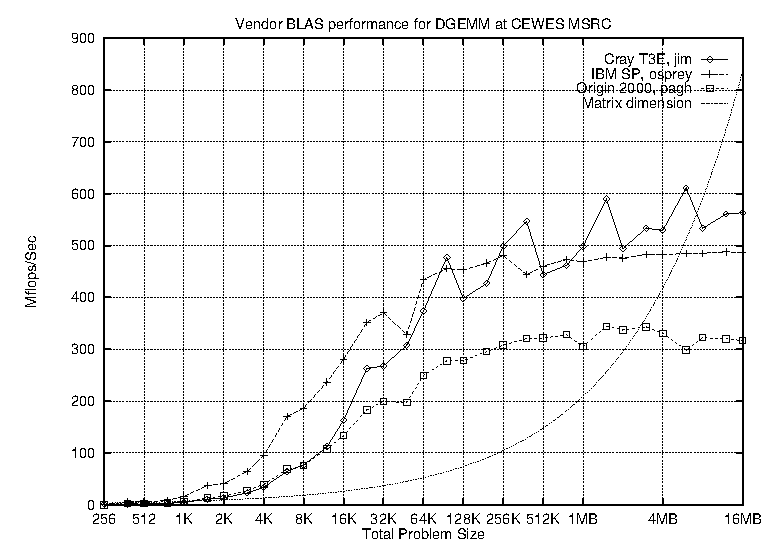
\includegraphics{pics/cewes_vdgemm.ps}}
\caption{Performance of Matrix-Matrix Multiplication with Scale}\label{dgemm}
\end{figure}
\clearpage
\newpage

Matrix multiply provides a lot of opportunity for cache reuse. By tiling the
matrices, the working set can be reduced to the size of cache and thus only
{\em capacity} misses are taken. For this reason, the performance of GEMM has long since served as a good indicator of a machine's {\em peak practical performance}. A machine with an adequate memory subsystem like the SP, can achieve
very high efficiencies, that is high percentage of the vendor's published MFLOP
rating. 

The reader should notice that clock speed and L2 cache size do not play as
critical a role in the performance of this routine as one might think. The 
spikes in the T3E's performance curve are due to the matrix dimension being
a multiple of the block size. For other cases, the GEMM routine must engage
in rather lengthy cleanup code. The small cache/line size of the T3E simply
exaggerate the performance loss. The SP, with it's large line size and ability
to issue 2 multiply-add instructions as well as a load/store per cycle does quite well, reaching approximately 90 percent efficiency. The Origin appears
to suffer from it's small cache line size and its inability to issue a 
load/store every cycle. The R10000 processor, like the Power2, can also issue
2 multiply-adds per cycle, but it appears to have great difficulty 
keeping those functional units busy. 
\section{Future work}

\begin{itemize}
\item Provide an option for measuring specific problem sizes and ranges.
\item Provide an option to specify the problem sizes in dimensionality.
\item Provide an option to specify the starting problem size.
\item Use specialized, high-resolution timers where available.
\item Add additional BLAS routines {\tt TRSM}, {\tt TRSV}, and {\tt SYR2K}.
\item Add parameters to tune the placement and padding of the arrays.
\end{itemize}

\section{References}

John Hennessey and David Patterson, {\em Computer Architecture, A Quantitative Approach}

{\tt http://www.netlib.org/blas}

\clearpage
\newpage

\subsection{Sample DAXPY - Numbers are erroneous}
\begin{figure}[Hht]
\centerline{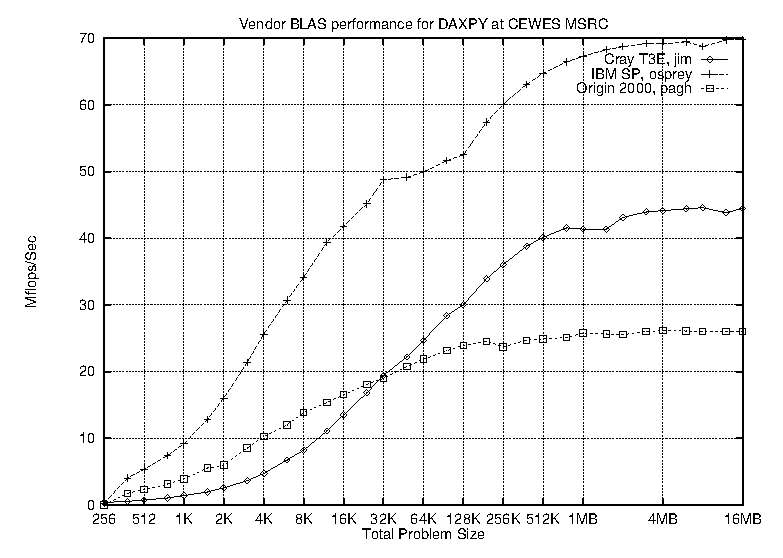
\includegraphics{pics/cewes_vdaxpy.ps}}
\caption{Performance of Vector Addition with Scale}\label{daxpy}
\end{figure}
\clearpage
\newpage

\subsection{Sample DGEMV - Numbers are erroneous}
\begin{figure}[Hht]
\centerline{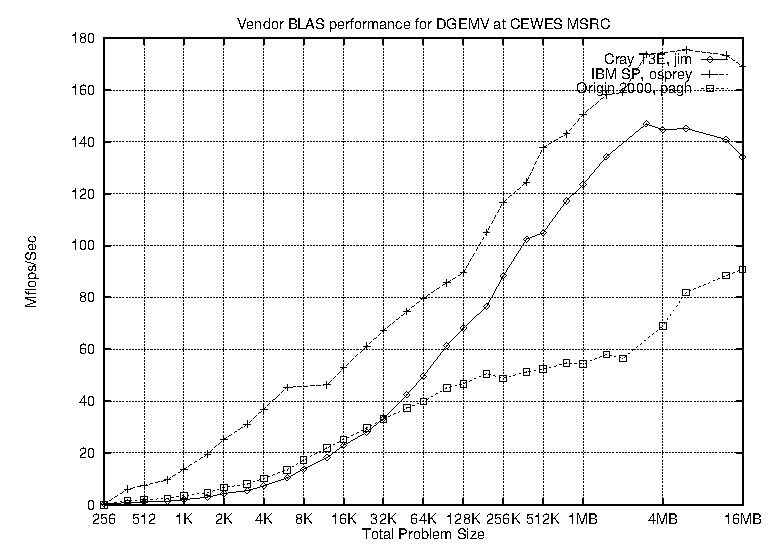
\includegraphics{pics/cewes_vdgemv.ps}}
\caption{Performance of Matrix-Vector Multiplication with Scale}\label{dgemv}
\end{figure}
\clearpage
\newpage

\end{document}

